\section{Why interpretability?}
Modern machine learning models based on deep neural networks are achieving remarkable performance in many fields. In comparison with classic machine learning technologies like decision trees, it is much harder to explain how these neural networks came to their conclusions, because they use thousands to millions of training parameters.

Especially in the medical imaging field, it is very important that algorithms not only generate a correct diagnosis when training the algorithm, but also show that they are using the same cues in images as do trained physicians. These cues are found and verified in scientific studies, and therefore are well understood and proved to be correct. A wrong diagnosis generated by a neural network reduce the confidence of physicans using the technology or can even be life threatening when used without professional supervision.

\section{Image classification}
In recent years, many methods for the interpretability of deep (convolutional) neural networks have been proposed, e.g. LIME \cite{ribeiro2016should}, RISE \cite{Petsiuk2018rise}, Grad-CAM \cite{selvaraju2017grad} or DeepLIFT \cite{shrikumar2017learning}.

\begin{figure}[h]
\centering
\caption{Examples of some interpretability methods for image classification \cite{visualattribution}}
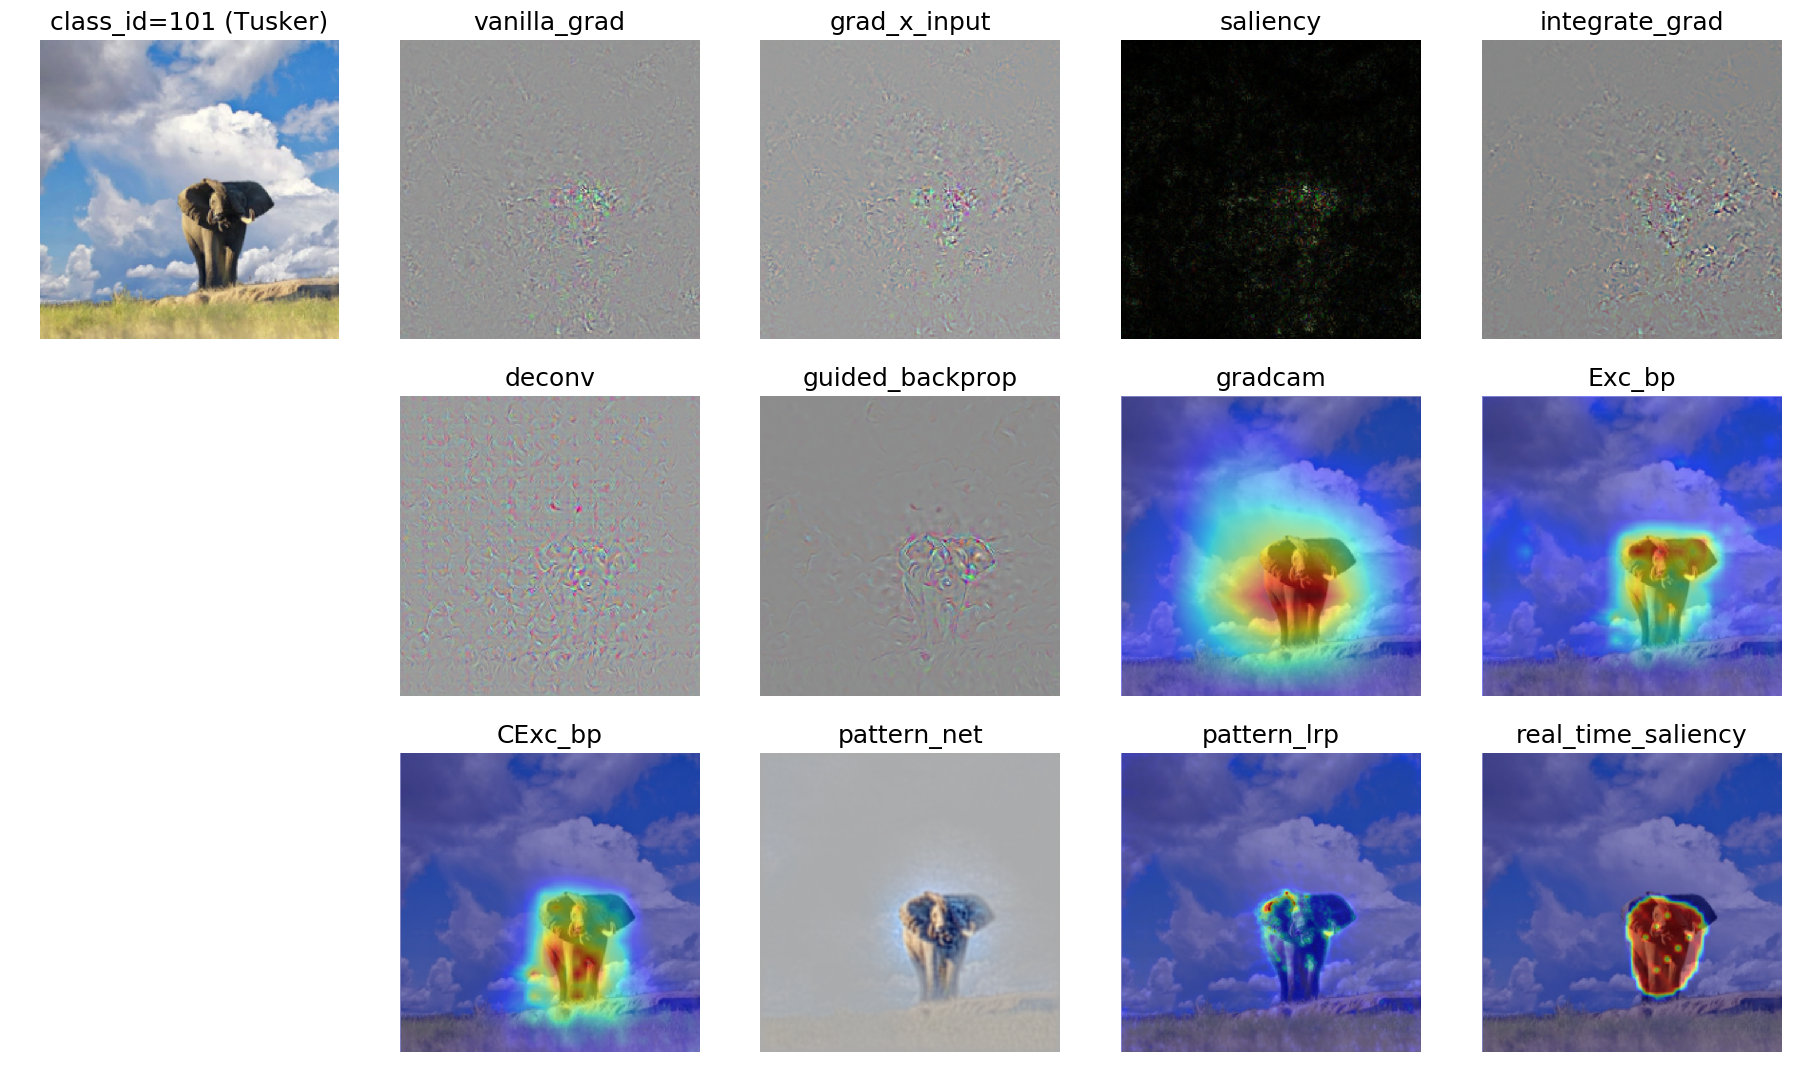
\includegraphics[width=14cm]{images/tusker_saliency.png}
\end{figure}

These methods focus on providing explanations and interpretability of classification problems for datasets like ImageNet \cite{imagenet_cvpr09} or MNIST \cite{lecun-mnisthandwrittendigit-2010}. Classification means that an algorithm can tell what is displayed on an image, e.g. if and what kind of disease is visible on a x-ray or MRI scan.

\section{Image segmentation}
Image segmentation is different from classification in the way that the algoriths do not detect what is visible on a picture, but instead mark a region (the segment) in an image where it thinks something is visible. For example in self driving cars, it is important to know where another car or a pedestrian is in front of the car is. 

In the medical imaging field, one applications is the segmentation of tumors in MRI scans.

\section{Interpretability on image segmentation}
The interpretability of image segmentation task is nearly inexistent. In many cases this is understandable, because the interpretability methods would generate an image very similar to the actual segment. For example, in detecting pedestrians for self driving cars, the interpretability method would just mark the pedestrian. Only in cases where the network has not yet reached a good accuracy, other pixels in the image would be marked by the method.

In other fields like medical imaging, it is possible or even desirable that a neural network looks at other parts of an image to decide if a part should be segmented. An example for this is the search for tumors on MRI scans of the human brain. The human brain is physically symmetric. When a tumor is growing on one side of the brain, the brain is no longer symmetric. A physician and possibly also neural networks can use this property to detect and segment tumors.

\section{Goals}
The goal of this thesis is to take the existing methods for image classification and modify them so they can work on image segmentation tasks. This includes the following tasks:
\begin{itemize}
    \item Research existing methods for image classification
    \item Asses if the found methods can be modified for image segmentation
    \item Modify the methods for image segmentation
    \item Build and train a neural network on the BraTS brain tumor segmentation dataset
    \item Apply the modified methods on the trained neuronal network
    \item Analyze, evaluate and discuss the results
    \item Build a reusable Python library so other developers can easily use our modified messages
\end{itemize}

The second goal is providing the customer with images and visualization for use in their teaching material.

See appendix A for the full requirements specification.

\section{Customer}
The customer of this thesis is Mauricio Reyes and his team from the medical faculty of the University of Bern. Mr. Reyes is head Healthcare Imaging A.I. This thesis should help him and his team of master and PHD students to better understand the models they are developing.

\section{Source Code}
The source code of the thesis is available on GitHub:
\begin{itemize}
    \item Thesis source code (mostly jupyter notebooks): \url{https://github.com/andef4/thesis-code}
    \item Python library source code: \url{https://github.com/andef4/interpret-segmentation}
    \item Latex source for this document: \url{https://github.com/andef4/interpret-segmentation}
\end{itemize}

All source code is licensed under the permissive MIT license.
